
\chapter{Approach and Requirements}
In order to conceive detailed use cases and a corresponding architecture, an explorative process had to be used. The initial overall objective was to create a general-purpose DDoS visualization system that focuses on data obtainable from DDoSDB datasets. In existing literature, one can find processes on how to derive an appropriate visualization for a defined problem, such as the following data analysis steps from Marty\cite{appliedsecurityvisualization}:
\begin{enumerate}
    \item Define the problem to become aware of which questions need to be answered by the final visualization.
    \item Assess the available data to determine how it can be used and how it might need to be extended.
    \item Parse and filter the available data to extract the relevant information.
    \item Determine which visual properties, such as shape or size are needed.
    \item Determine the view of the graph that was created in the previous step. This includes transformations such as scale or zooming.
    \item Interpret the graph and answer the initial question.
\end{enumerate}

Since this process is targeted at solving a specific problem and our objective was the development of a general-purpose visualization system, we adapted it as is described in the remaining sections of this chapter. First, we analysed the information that can be extracted from various network captures from DDoSDB. This also included the determination of their scale and possible tools for data extraction. The outcome of this step was a general understanding on how the data needs to be parsed, aggregated and or filtered to create a general-purpose visualization system. This constitutes a "bottom-up approach" where we first analyse the data and parse it in the most generic way,  enabling the information to be used with as many visualizations as possible while still maintaining technical feasibility for larger datasets.

The requirements for the solution were defined after the literature survey was conducted and discussed with the project's supervisors experienced in the field of visualization and DDoS Attacks.
Given the requirements to such a system and the understanding of available information and scale of the data sets, we then created the initial architecture.

\section{Analysis of Data Sets}
Before defining detailed use-cases, available data was explored to determine feasible requirements, visualizations and implementations. To be more specific, a proof of concept data mining tool was built to answer the questions that needed to be cleared before progressing. The following subsections describe the questions that were supposed to be answered by the Proof of Concept and their results. With these results in hand, an initial brainstorming session about possible use cases done we were able to synthesize all information. The result is the use cases that are supposed to be as abstract as possible to be in line with the overall objective of building a general-purpose platform whose prototypical implementation can be considered technically feasible.
The scope of the POC was to write a data miner that can provide at least the same functionality as can be obtained from the fingerprints available in DDoSDB.

\subsection{Libraries and Tooling}\label{librariesandtooling}

\textit{What libraries exist and which features do they provide?}   

   Different tools and libraries were evaluated, such as tsflow, a CLI tool, node\_pcap, a JavaScript based wrapper around libpcap, and pkts, which is a parser written purely in Java.
    The Java library seemed to provide the best performance, but for simple prototyping the Node.js based library was chosen. It provided parsing of protocols up until the application layer (app layer not included?) and heavily relies on libpcap. Support for stream processing in Node.js and the event-driven nature of JavaScript made the implementation feel quite "natural" and easy to read.
    Using node\_pcap, it was possible to create the same information as provided in the DDoSDB dataset. Initially, we suspected to run into performance problems, especially when using very large datasets, which turned out not to be the case. This was due to the ease of implementation using stream processing which would make the POC scale easier with large sets. The duration it took to mine a data set was shorter than initially expected. This was tested by profiling the application when mining the largest dataset we could find on DDoSDB. This revealed that it only took seconds and that a majority of time was spent in the native libpcap module. This can be explained in that node\-pcap is merely a wrapper around libpcap. Figure \ref{fig:profiling} shows the result of profiling the miner. We thus conclude that node\_pcap provides all required functionality and that writing the miner in a way that it scales to larger datasets will be technically possible.
    
    \begin{figure}[]
    \centering
    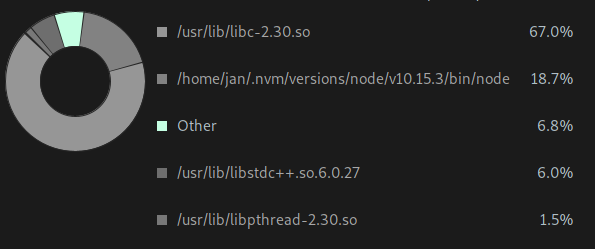
\includegraphics[width=10cm]{images/profiling.png}
    \caption{Profiling the data miner with a 15MB network capture as input.}
    \label{fig:profiling}
\end{figure}


\subsection{Information granularity?}
\textit{What information is contained in the network capture data sets? Which protocols and levels are sensible to analyse?
}

As a source for possible datasets, the DDoSDB database was chosen. The reason for this are the features it provides as stated in section \ref{ddosdb}. The main benefit was direct access to network capture files that are already classified and in various sizes. This made it easy to see which information can be obtained in different attacks, such as for example, the payload of an ICMP packet. Since it is very simple to create a network capture of a "normal state" it was simple to compare the analysis of both cases.
Using the network capture files and a WHOIS service with the implemented proof of concept, we were able to recreate the fingerprints from DDoSDB along with some additional information. The remainder of this section describes the data that can be extracted and an assessment if and how it is useful to collect for a visualization system:

\begin{itemize}
\item \textbf{PCAP}:
The first packet is a PCAP wrapper around the network-access level packet. It contains information such as \textbf{packet length} and a \textbf{timestamp} in seconds and microseconds. It is worth to note that this data needs to be interpreted on the place where it was captured.
Both of these properties are important to gather in order to compute the average packet length and attack start and duration.

\item \textbf{Network Access Layer}: 
In the payload of the PCAP packet, one usually finds an Ethernet packet. Other network-layer protocols would be possible but only Ethernet packets were observed in the network captures.
The following information can be extracted from Ethernet packets:
(i) Destination and Source MAC addresses, (ii) Network-layer Protocol and (iii) VLan ID.

Since the information is very low-level and does not convey important semantics about any of the most frequent DDoS attack types we don't consider any of the information useful to store, except for the Internet protocol that would be considered in the next subsection.


\item \textbf{Internet Layer}: 
This was the first layer where multiple protocols were observed, naturally those would be IPv4 and IPv6. The network captures within DDoSDB were almost entirely based on IPv4 which is why this was focused on:
(i) Source and Destination Address, (ii) Version, (iii) TTL, (iv) DiffServ, (v) Length, (vi) Transport-Layer Protocol and (vii) Checksum.

Except for checksums and transport-layer protocol, which was considered on the next layer, all properties could be sensible to mine.
For some attacks the number of involved source addresses was very large, so large that fingerprints from DDoSDB would easily be larger than five megabytes. The problem with that is that it is difficult to work with in a front-end web application and it would be hard to visualize. For datasets that exceed some threshold of number of IP addresses aggregation would likely be required. This aggregation could be done based on arbitrary prefix aggregation, country or autonomous system.
Other properties that are also sensible to aggregate would be TTL and length.

\item \textbf{Transport Layer}: 
In the transport layer, two protocols were frequently observed: UDP and TCP.
Common to the two are the two fields (i) Source and Destination Port and (ii) Checksum.
The packets using the TCP protocol also showed the following fields: (i) Acknowledgement Number, (ii) Sequence number, (iii) Header length, (iv) All six single-bit flags, (v) Window size and (vi) Urgent Pointer.
Source and destination port information is valuable data to gather information on the application protocol being attacked. The flags would also be easy to aggregate over and give insight over the TCP state.

\end{itemize}

\subsection{Application layer}
The library that was used to parse packets does not contain a parser for application-level protocols. This means that to analyse this layer one has the protocol number and a buffer containing the payload. Perhaps it is already enough to aggregate over the type of protocols used. However the final implementation should definitely be easily extendable with new parsers for such protocols. For example, Node.js offers a performant and widely used HTTP parser which could be used to further gain insight about the application-level attack.
     
\subsection{Scale and Schema of data}\label{scaleandschema}
\textit{Will the size and schema of the data introduce challenges with respect to visualizations? Can some technical challenges be determined?
}

    The reason why this question needs to be answered before designing visualizations is that depending on the size and distribution of the attributes needed to be visualized, the visualization will either provide little value or be technically difficult. For example, consider an attack with 100'000 source IP addresses. Storing and fetching these addresses from a server to a web application will be taxing. Even if this were possible, there will hardly be a visualization that will provide insight while visualizing all 100'000 IP addresses. The answer to this question should define if and how aggregation of such attributes needs to be done.
    This is a technical challenge that can be taken for granted since network captures are technically unbound in size. This will also imply technical challenges for the mining of the source data since not the whole source and analysed data can be kept in memory.
    These challenges were observed while implementing the proof of concept. We assume that the following countermeasures will become important:
    \begin{itemize}
    \item     Applying \textbf{Big data techniques} to mine the source data will be very important to guarantee that the data miner is technically capable of handling very large network capture files.
\item Looking at the fingerprints of the larger network captures in DDoSDB reveals that some of these JSON files are multiple megabytes in size. This is both technically challenging to transfer and render and also hard to interpret. However, not only the size of these summaries is a problem, the fact that all information is contained in a single JSON file would lead to overfetching when used for different visualization. Overfetching refers to the problem of having to retrieve more data than being required by the client. Our solution to reducing the size and getting rid of overfetching is to create different resulting files for different visualizations. In a sense we would try to "\textbf{fan out}" the results over multiple files for improved scalability. For example, this could mean that for a time-series analysis of an attack we would create fixed-sized intervals and then create JSON files for each time interval. For other visualizations that would deal with more abstracted information we would also create single JSON files that have the only purpose to be used in that visualization. For example, a bar chart visualization showing the top five autonomous systems used in an attack would only have to fetch a very small, dedicated JSON file containing said information.
\item Another solution to the aforementioned dilemma with very large results is to \textbf{aggregate} them. Ideally, this should be possible in a dynamic and user-defined way. For example, if an attack is executed from five source IP addresses, then this is technically possible and sensible to store as result and show in a visualization. However, for hundreds or thousands of IP addresses either this visualization should be disabled or the underlying data could be aggregated to larger prefixes.
\item To enable the threshold where data will be aggregated more aggressively, such a \textbf{user input} has to be implemented into the front end of the web application.
\item Using a WHOIS service to query additional data about the source IP addresses does not scale up if more than a few thousand IP addresses need to be analysed. This is due to many WHOIS service providers being unwilling to deal with bulk requests of this size. Additionally, such requests would increase the duration of the data mining, since it has to be transferred over the network. A local database needs to be considered as described in \ref{enrichingthedata}
\end{itemize}
    
    \subsection{Enriching the Data}
\label{enrichingthedata}    \textit{Given the information that can be extracted, how can it be enriched? Which information makes sense to complement the network capture information with and how can it be obtained?}
    
In order to rebuild the functionality provided by the DDoSDB data miner, we need to provide the country and autonomous system number (ASN) for each source IP address.
In the proof of concept implementation we used a WHOIS service provided by Team Cymru. This service supports bulk requests for WHOIS requests but is only willing to answer requests containing "(..) a few thousand" IP addresses \cite{teamcymru}. This along with the latency introduced by fetching the results over the network make this solution impractical. For this, we intend to use the Geolite2 databases which are often used for geolocation of IP addresses. These datasets are interesting to us since they can be used locally and they have different datasets through which we could retrieve the ASN, country, city and belonging prefix for a source IP address \cite{geolite2}.

    
    \subsection{Aggregating the Data} 
\textit{Given the information that can be extracted, is there a need for it to be aggregated and if yes, how it it done? 
}    

Section \ref{scaleandschema} described the necessity to aggregate in order to improve technical scalability and to make the visualizations sensible.
To visualize information with little abstraction, such as for example the source IPs for a certain time period, we will create a small data set containing just the relevant properties for that time interval.
For information with higher abstraction, such as visualizing overall metrics, we follow the same strategy of creating a dataset for the visualization.
    \subsection{Fitting visualizations}
\textit{Given all the information that can be obtained, which visualizations are sensible?
}

We already established that the datasets need to be decoupled depending on visualization. To build a general purpose visualization platform, it would be a good strategy to build a data miner that can easily be extended and then build visualizations and parsers for the most common attack types.
    \subsection{Constraints} 
\textit{Which constraints on the user input make sense? Which data sets make sense (e.g. location of recording)?
}

If the application can deal with large datasets, there should still be a limit for the size of input files since we don't know in which setting the application would be used. We think it makes sense to allow a user to define such a threshold in the application. Other constraints that are related to the visualizations, for example hiding certain outliers should be considered when designing the visualization.
In a first step it makes sense to write parsers only for network capture files, ideally from the DDoSDB database.
    
    \subsection{Frequent problems described in literature} 
    \textit{Literature describes that frequent problems are "Incomplete Information" and "Source / Destination Confusion". Are such problems relevant and if yes, how can they be mitigated?}
    
    Detecting whether a dataset is incomplete may cause difficulties, since the proposed solution is not supposed to act as a classification or intrusion detection system. Since this data was already pre-processed by the DDoSDB\-cli, we  work under the assumption that a pruned network capture file is used as input. 
    What is likely to happen and feasible to detect would be errors introduced when aggregating or extending the data. This would need to be indicated to the user somehow. For example, consider the case where we compute the top five autonomous systems used for an attack. If some of the IP addresses found in the parsed network captures cannot be assigned to an autonomous system, this information needs to be made aware to the user. Otherwise, the information visualized will be distorted.
    The source destination problem is already mitigated to a certain degree since the destinations in the network capture files have been anonymised. What remains important is keeping a consistent naming and documentation throughout the data model up until the user interface. For example, this will require that the axes of the diagrams are labeled appropriately.
    
\section{Use Cases}
\label{sec:usecases}
To shape the direction of this project, use cases were created, based on three stakeholders we defined: \emph{Researcher}, \emph{Network Operator} and \emph{Professor}. In the tables \ref{table:us-researcher}, \ref{table:us-operator} and \ref{table:us-professor} the defined use cases have been categorized by role and in \ref{table:us-general}, use cases that feature multiple roles were presented as well.

\begin{table}[]
\centering
\begin{tabular}{|p{1.6cm}|p{12cm}|}
\hline
\textbf{ID} & \textbf{Description} \\ \hline

UC-G-1         & As researcher, professor and network operator, I want to upload a PCAP file to have it analyzed and  visualized by the application. PCAP files should be accepted from DDoSDB or directly from network capture software.\\ \hline
UC-G-2         & As a researcher and network operator, I want to be able to extend the platform by writing parsers/analysers for additional file types\\ \hline
UC-G-3         & As a researcher, professor and network operator I want to be able to replay an attack using configurable time controls such as play/pause buttons or a time line. To inspect an attack in detail.\\ \hline
UC-G-4       & As a researcher and network operator, I want the application to work with very small and very large data sets. This will likely involve that the application is aware of the size of data sets and its effects on visualizations \cite{appliedsecurityvisualization}. For example, the visualization of a all source IP addresses will require the aggregation into classes or prefixes if there are hundreds of thousands of addresses.\\ \hline
UC-G-5         & As a researcher, professor and network operator I want the uploaded data sets to be persisted on the application, so I can have the same data sets across multiple sessions.\\ \hline

\end{tabular}
\caption{Use Cases affecting multiple stakeholders}
\label{table:us-general}
\end{table} 

\begin{table}[]
\centering
\begin{tabular}{|p{1.6cm}|p{12cm}|}
\hline
\textbf{ID} & \textbf{Description} \\ \hline

UC-P-1         & As a professor, I want to use the application from a browser without installing additional software, because this way I can access the service from various devices.\\ \hline
UC-P-2        & As a professor, I want the application to come bundled with data sets that clearly show different attack types to show students what they look like and how they differ in appearance.\\ \hline
UC-P-3        & As a professor, I want to be able to let students detect the type of attack by having the same packet capture plotted on different visualizations.\\ \hline
UC-P-4       & As a professor performing network security workshops, I work with different customers. The hardware and software that they use varies greatly which is why the application should work with all modern browsers and on slower hardware.\\ \hline
UC-P-5      & As a professor that presents the visualizations in presentations and lectures, I want to save and retrieve my setups and retrieve them at a later point in time, so I don't have to reconfigure a setup from scratch every session\\ \hline

\end{tabular}
\caption{Use Cases representing a Stakeholder from an educational background, e.g. a professor.}
\label{table:us-professor}
\end{table} 



\begin{table}[]
\centering
\begin{tabular}{|p{1.6cm}|p{12cm}|}
\hline
\textbf{ID} & \textbf{Description} \\ \hline

UC-R-1        & As a researcher, I want to be able to host the application on my own machine and use it in a private environment, so I can make changes to the platform and test them.\\ \hline
UC-R-2         & As a researcher, I want to be able to extend the platform by extending the visualization capabilities of the application\\ \hline
UC-R-3        & As the researcher that hosts the platform, I want to access preferences of the application using an admin panel. For example, the maximum file upload size can be defined.\\ \hline
UC-R-4       & As a researcher, I want to be inspired to try new visualization techniques, since this is often required to find new patterns in network logs \cite{appliedsecurityvisualization}. This requires that one can easily add, combine or adapt new visualizations for an existing data set to find new patterns in network logs as well as one can quickly try different visualizations for the same attack.\\ \hline
UC-R-5       & As a researcher that  wants to use the visualizations in papers, I want to be able to export the visualizations to PDF and image formats.\\ \hline
UC-R-6       & As a researcher, I want that visualizations are categorized by the attack pattern which they are likely to indicate and the required technical understanding as described in UC-N-6. It should be easy to filter and select these visualizations.\\ \hline
UC-R-7      & As a researcher, I want to get certain statistics that span over multiple attacks. For example, given a set of network captures, what was the most commonly used protocol?\\ \hline
UC-R-8      & As a researcher, I want to have an overview page for each dataset where I can see general information about the set such as description and high level statistics.\\ \hline
UC-R-9     & As a researcher associated with DDoSDB, I want that the system can visualize the fingerprints generated by the ddosdb\_cli. This will likely require that the data model from those fingerprints is used and optimized so that it works for visualizations. \\ \hline
\end{tabular}
\caption{Use Cases expressed by a researcher}
\label{table:us-researcher}
\end{table} 

\begin{table}[]
\centering
\begin{tabular}{|p{1.6cm}|p{12cm}|}
\hline
\textbf{ID} & \textbf{Description} \\ \hline

UC-N-1         & As a network operator, I want the system to prioritize support for packet capture files, rather than network flow data, since packet captures provide a much more raw and unfiltered overview of an attack. \\ \hline
UC-N-2        & As a network operator, I want to be able to feed network data directly into the application, to monitor my network in real time.\\ \hline
UC-N-3        & As a network operator, I want to upload other file types, since my packet capture system uses a different file structure than PCAP.\\ \hline
UC-N-4        & As a network administrator, I want to have source IPs clustered by Attributes such as ISP, country or Prefixes to have a better overview of where an attack came from. This implies that additional information to the network capture is gathered.\\ \hline
UC-N-5         & As a network operator, I want to be able to aggregate metrics of a PCAP file, such as the rate of incoming packets per second or the number of incoming connections. to find out high level information and conclusions about an attack as a whole.\\ \hline
UC-N-6        & As a network operator, I want to switch between simple visualizations with limited information and more complicated ones that are more detailed, so when I have to inform a higher up who is not very technically skilled I can present him or her simple visualizations that are easily understood.\\ \hline
UC-N-7       & As a network operator, I want a visualization software that is agnostic to the type of attack or location where the attack was recorded. This stands in contrast with other tools such as Firewalls that have implemented visualizations as an afterthought which are specialized \cite{appliedsecurityvisualization}.\\ \hline
UC-N-8       & As a network operator responsible for reporting to (non-technical) management, I want very high-level visualizations for all types of attacks. This is a requirement since one often has less than 60 seconds to get a message to a non-technical person \cite{appliedsecurityvisualization}. This will require aggregations as described in UC-G-4 and UC-N-4. \\ \hline
UC-N-9       & As a network operator responsible for the historical analysis of attacks, I want to have detailed visualizations targeted at technical audiences, to draw conclusions about potential threats that might affect our network \cite{appliedsecurityvisualization}.\\ \hline

\end{tabular}
\caption{Use Cases expressed by a network operator}
\label{table:us-operator}
\end{table} 

As mentioned in UC-G-4, it is important that the application can handle small, as well as very large data sets. This requires that, depending on the visualization, thresholds have to be set for certain attributes that define when it will be clustered or used differently in a visualization. For example for smaller data sets it might be possible to draw all source IPs and their hosts, but for a larger set it may require a lot of CPU power that results in a visualization that it illegible and unnecessarily complex. This fact influences the way we pre-process data sets in order to have them visualized in the application as fast as possible. Another feature that is affected of this selective pre-processing, is the toggle that switches between simple visualizations only and more detailed and technical views. For a non-technical user that wants a broad overview of an attack, we assume that 1) the user is less inclined to wait until a visualization has loaded and 2) simple charts, such as bar charts and graphs that display precalculated metrics will suffice. This goes well in hand with our problem of differently sized data sets and the need of calculating metrics in advance.

\footnotetext{RQ 5: UDP floods and HTTP-based attacks have been the most common type of DDoS attacks by the end of 2018\cite{hostingtribunal.com}.}

\section{Components and Mockups}\label{components}
The following section will describe the proposed functionality of our solution and its relation to the use cases outlined in \ref{sec:usecases} using component descriptions. The possible actions a user can make inside a specific component will be presented. To further illustrate the functional design of the application, mockups and wireframes are shown along with the component descriptions. When a feature or functionality is derived from a use case, the appropriate use case from section \ref{sec:usecases} is mentioned in brackets.

\subsection{Startup and Login}
When a user opens the application, either hosted locally or via a public URL [UC-R-1], the welcome screen is shown. It features a brief introduction to and description of the application and project. Below the introduction a brief paragraph is shown that explains how our solution extracts data from data sets, as well as a paragraph explaining the dashboarding functionality. Additionally, a github link is provided, so that interested people can clone or fork the source code. 

\subsection{Navigation Bar}
Always present on the platform is the navigation bar, that allows switching between the three main tabs of the application. The first tab being \emph{Home}, that shows the aforementioned welcome screen. The second tab hosts the \emph{Dashboard} tab, which is where the data sets can be opened and visualized after they have been uploaded and analyzed. The third tab is the \emph{Datasets} tab, where all the currently uploaded and analyzed datasets will be visible [UC-G-5]. From there, the individual data sets can be opened on the \emph{Dashboard.}

\subsection{Dashboard}
The \emph{Dashboard} is where a user can open visualizations for the uploaded data sets. A mockup for it can be seen in Figure \ref{fig:dashboardmockup}  Elements are freely movable, so that a user can configure a formation of multiple visualizations to fit his needs [UC-R-4]. These setups can be stored and retrieved at a later point in time [UC-P-5]. Components of the \emph{Dashboard} are a \emph{Grid}, \emph{Data Set Tiles} and \emph{Visualization Tiles}. At the bottom right of the \emph{Dashboard} a \emph{Floating Action Button} hosts additional functionality for the grid, such as filters and the option to save and restore setups.

\begin{figure}
    \centering
    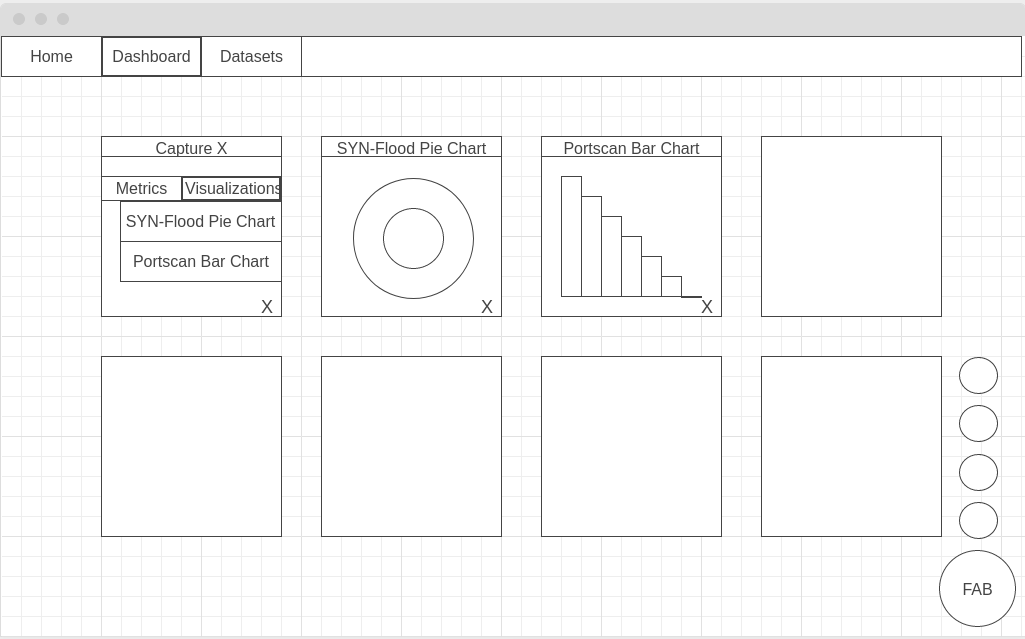
\includegraphics[width=16cm]{images/dashboard_mockup.png}
    \caption{A mockup of the \emph{Dashboard} page of the application}
    \label{fig:dashboardmockup}
\end{figure}

The main component of the dashboard is a dynamic \emph{Grid} that can be filled with two types of tiles, \emph{Data Set Tiles} and \emph{Visualization Tiles}, that automatically snap to the grid's cells and display information inside them. The width of the grid, in terms of columns, is variable, depending on screen size with a maximum number of 4 columns. The number of rows is dynamic, depending on the amount of tiles placed in the grid. Once enough tiles have been placed on the grid, so that it fills the screen, the grid becomes scrollable.
A user can perform different actions with the tiles placed on the grid, with the grid automatically reacting to a change. Tiles can be dragged from one cell to another, resulting in an automatic rearranging of the tiles, should it be placed in a cell that is already used by another tile. If a specific tile supports it, it can be increased in size, e.g. to take up two columns in width instead of one, with an automatic rearrangement of other tiles, to make sure a cell is only used by one tile at most. Additionally, grid items can be filtered by data set, so only certain tiles are visible at one time.

A \emph{Data Set Tile} represents a dataset that has been uploaded to and processed by the application. It displays the dataset's name, a short description of it and the main area of the tile that features two tabs; one for displaying \emph{Metrics} and one for displaying a list of possible \emph{Visualizations} for that dataset. When opened on the grid, a randomized hash-icon is assigned to this dataset tile and the visualizations it opens, to be used for identification purposes. 
The \emph{Visualizations} tab contains a list of visualizations, grouped either by the attack type they are most likely to be able to identify or by the type of visualization [UC-R-6]. For example, under a \emph{Portscan} entry, one can find visualizations that display the most commonly used ports on a bar chart [UC-P-3].
After selecting a visualization, it is opened as a visualization tile on the grid spanning one or more cells, depending on the visualization’s minimum size, as close as possible to the originating data set tile. In order to make clear to a user to what dataset a visualization tile belongs, the hash icon at the top of the tile is identical to the one on the originating \emph{Data Set Tile}. Another button on a \emph{Data Set Tile} is a \emph{Close} button, represented by an "X" character, that closes that tile.

The \emph{Visualization Tiles} differ in functionality between the types of visualizations they contain, but all feature a title at the top describing the visualization. As mentioned above, the hash icon at the top of the tile will be the same as the originating data set tile, making it easy to distinguish which tiles belong to the same data set. This includes customizable filters or the option to close that visualization tile. the actual visualization is centered in the tile, taking up the majority of the tile. Every \emph{Visualization Tile} features a download button that lets a user export said visualization as a PNG, to be used in reports and documents [UC-R-5]. Similarily to the \emph{Data Set Tile}, the \emph{Visualization Tile} has a \emph{Close} button that removes the tile from the grid.

After clicking on the \emph{Floating Action Button} in the bottom right corner, a Speed Dial [source] menu is opened featuring functionality for the currently opened setup as clickable elements in a list.
\emph{Save Setup} lets a user store the currently configured dashboard with a name, to be opened at a later point in time by clicking the \emph{Restore Setup} entry [UC-P-5], which opens a modal containing a list of all saved setups. The setup includes data sets, visualizations, position and size of all tiles, as well as settings for the individual visualization tiles. \emph{Clear Dashboard} lets a user close all tiles at once and start over with a fresh unconfigured dashboard. When deleting a dashboard that has not been saved, the user is asked if they want to save it before deleting. The \emph{Filter By Data Sets} entry opens a modal dialog that lists all currently opened data set tiles. When clicking on a specific data set on that list, the visualizations from that data set become opaque, making other tiles stand out. Lastly, the \emph{Save to PDF} entry lets a user export the current dashboard as a PDF file, with all tiles rendered for document use [UC-R-5].

\subsection{Data Sets}
The Data Sets page lists all uploaded and analysed datasets on the platform. From here, the datasets can be compared and inspected, and opened on the \emph{Dashboard}. Component-wise the page consists of a list of \emph{Data Set List-Items} and an \emph{Upload} button at the bottom right corner. The list is sorted by upload date of the data sets in descending order and is scrollable, once enough data sets have been uploaded [UC-G-5].

The individual \emph{Data Set List-Items} represent an uploaded and analysed data set on the application. On the left hand side of the item, user-entered information, such as the data set's name and description, is displayed. On the right hand side, file-related information, such as the upload date, analysis status and file size is displayed. At the bottom of the item are two buttons, as well as an \emph{Expand} arrow. \emph{Open}, imports the data set into the dashboard, meaning that a new data set tile will be opened in an empty tile in the dashboard's grid. After performing this action, a notification badge appears at the bottom of the page, indicating that the data set was successfully opened. The \emph{Delete} button prompts the user for confirmation, whether the specific data set should be deleted from the application. Confirming the action results in the deletion of the original uploaded data set, as well as all derivative data calculated from it. When expanding the item, calculated metrics will be listed, as well as the derived data files used for visualizations [UC-R-8, UC-N-5].

Lastly, the \emph{File Upload Button} allows a user to upload PCAP files. After clicking on it, a modal dialog appears where the file can be selected from disk. A name and description can be given to the file, so that it can later be identified. After all information is entered, the upload button in the lower left corner can be clicked, after which the file will be uploaded. After successful uploading, the user receives a notification at the bottom of the page [UC-G-1].

\section{Architecture for DDoSGrid}
Section \ref{components} has shown how the use cases will be met from a functionality point of view. This section deals with the architectural choices that were made to enable said functionality. First, we will outline our general approach to mining and visualizing DDoS attacks and then we will describe each component and its purpose. This architecture will be evaluated in the next sections, where a concrete design is outlined that fits this architecture.

\subsection{Overview}
Figure \ref{fig:architectureoverview} visualizes the main components that we propose to be built and their relationships. The relationships are shown as directed arrows indicating the flow of data. Our architecture can be separated into two logical parts, the first one being the User Layer, which deals with the handling of user input and the visualization of results. The second part is the Data Layer, providing storage and analysis of the raw PCAP files and their results. The next paragraphs will outline the purpose and relationships of the individual components.
\begin{figure}
    \centering
    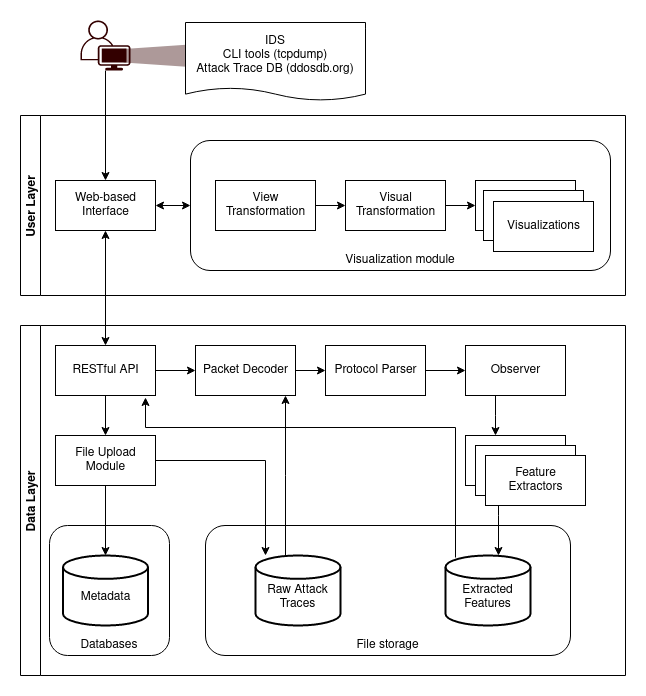
\includegraphics[width=16cm]{images/Highlevel-approach.png}
    \caption{Architecture overview of our proposed solution.}
    \label{fig:architectureoverview}
\end{figure}

\subsubsection{Web-based Interface}
The Web-based Interface is the user's main entry point and handles all matters that directly affect the user. This spans the handling and distribution of user input, for example the manipulation of the visualizations or the upload of the raw PCAP files. It therefore interacts with the visualization subsystem which is also in the User Layer and it interacts with the Data Layer through a single RESTful API.

\subsubsection{Visualization Module}
The Visualization module renders the result produced by the analysis modules as a diagram. This module contains three components which closely work together and may even be implemented as one software module, which is why they will be described together.
First, the View Transformation component receives the results of the Feature Extraction process through the previously mentioned RESTful API. It then transforms the properties of the data structures into fitting visualizations. For example, by mapping the number of packets contained in a result to the values for a y-axis of a bar chart.
This configuration can then be further manipulated by doing Visual Transformation which can change the way how these properties are shown. For example, given that a user wants to zoom out, it would aggregate certain data points that would be on the y-axis of a Bar Chart.
Finally, with this configuration a set of visualization components can plot the data using different visualization techniques. For example, a set of TCP ports and their number of occurrences could be plotted using a bar chart or a pie chart. This module contains the software modules that are able to produce the diagrams.

\subsubsection{RESTful API and File Upload Module}
Looking beyond the User Layer, we only see one module being exposed, namely the RESTful API. This component exposes all the functionality of the Data Layer and orchestrates the analysis process and the storage of data.
It accepts PCAP files and metadata about the capture file being uploaded from the Web-based Interface. Thus ensuring that the raw PCAP files are being stored appropriately and that the metadata is stored in a database. This would cover properties like the upload date, file size, analysis status and so on.
This uploading procedure has to be handled with care since PCAP files have no maximum size. Therefore, one needs to implement this module in a way that does not deplete memory resources.
Once the user requests the uploaded capture file to be analysed, this module shall orchestrate the analysis of different feature extractors over a stream of decoded packages. Finally, it retrieves and stores the results of the analysis and updates the metadata associated with the input file.

\subsubsection{Packet Decoding}
The Packet Decoding module reads a PCAP file supplied by the RESTful API and parses packets using a variety of protocol parsers. Once a packet has been decoded, it allows clients to be notified about the presence of the packet. This API should allow for an Observer pattern-like access of independent clients to the decoded packet. The actual set of subjects the clients may observe depends on the supported protocols and their abstractions. For example, after the Packet Decoder has parsed an Ethernet packet, it can emit the packet to clients observing the subject \textit{Ethernet} and \textit{Layer-1-packet} where the latter is an abstraction of the former. The purpose of these three modules is to allow independent feature extractors to observe packets of some protocols so that they can analyse them without fetching packets they do not need or without being affected by other feature extractors.

\subsubsection{Feature extractors}
The previous paragraph has outlined how a set of independent feature miners can access packets of a very specific protocol or abstraction. This allows for independent feature extractors that focus on producing a visualization result for one attack type. For example one implements an autonomous feature extractor for the visualization of a possible SYN-flood attack and an additional miner for a DNS amplification attack. The first miner observes packets being emitted in TCP protocol and the latter observes an application-layer protocol. Then, they extract relevant features from the packets and finally store them for analysis. For example, the SYN-flood miner looks at the TCP flags indicating connection state, taking note about the distribution of connection states over all observed packets. Finally, it will format the results for visualization and indicate how they can be visualized.

\subsubsection{Storage}
There are three modules that provide persistence for the modules described before. The first one is the metadata database, where information like dataset names or upload dates are stored. The other two are structured file system modules that store the input PCAP files supplied by the user and the resulting analysis results.

\chapter{Design and Implementation} \label{chapDesign}
The previous chapter introduced a high-level view on how our approach is supposed to work. This chapter explains the prototypical implementation of that approach to prove its feasibility. For this prototypical implementation we simplified some parts of the architecture, however this was done with compatibility and portability of the modules to their initial concept.

\section{Prototypical Design} 
In order to build the system in an iterative manner we derived a simpler version of the architecture described in the previous section. This architecture is a pure simplification that is still compatible and should allow quicker prototyping and gathering of feedback. 

To build a minimal version that can show the systems capabilities and gather feedback there would only be one service exposed and operated by us. This would be a Node.js based Express.js application that contains the RESTful API, a static webserver for the analysis files and an embedded database for metadata. The actual miner would be built in a separate Node.js module and run in the different process. This is necessary so that the main thread is not blocked and can still answer to HTTP requests. Since in this version we are the only developers writing analysis modules we can easily optimize these modules so that the overall memory constraint withing Node.js is not an issue. This configuration also only requires one file storage volume for both database and analysis files. If one were to optimize and extend the system one could pull the modules apart into their own Docker containers and replace some of the parts such as the Webserver and database with third-party technology such as nginx and Mongodb.
For convenience, the front end application can directly be hosted by GitHub pages which provides fast integration into the continuous delivery process. Since GitHub pages provides free https certificates and has CORS configured properly, it provides all requirements for the front end web application. A view on this deployment is shown in figure \ref{fig:deploymentviewmvp}.

\begin{figure}
    \centering
    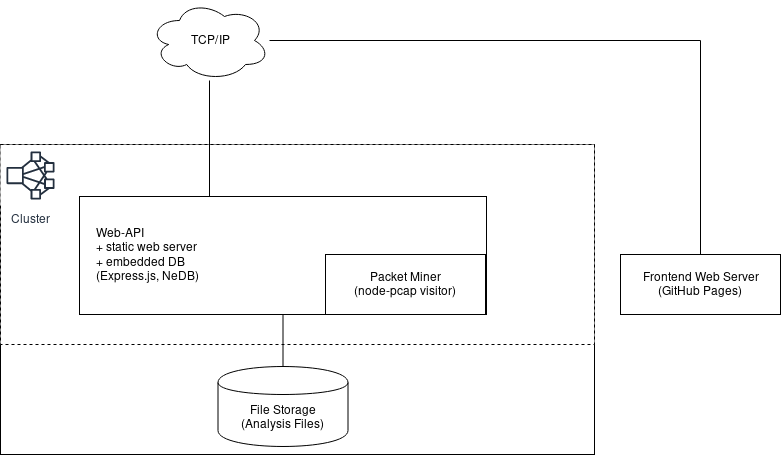
\includegraphics[width=16cm]{images/deploymentviewmvp.png}
    \caption{Deployment view view of the minimal architecture.}
    \label{fig:deploymentviewmvp}
\end{figure}

\section{Back End Development View}
The previous chapter has already described which services exist in the back end and which features they provide. Since this architecture contains both bespoke parts and third-party software, we will not describe the design of their internals but rather just outline the most relevant questions and challenges that were faced when building the architecture.

\subsection{Network capture decoding}\label{networkcapturedecoding}
The biggest decision when implementing the packet parser was which library to use for network capture decoding. The evaluation of possible libraries was explored in the beginning as described in \ref{librariesandtooling}. The findings of our exploration was that we would either use the Node.js based node\_pcap library or a Java-based library. Since this module is probably the most important for our project this decision became central since it would decide the overall platform used. For example, we would rather not build the miner in Java and the Web API in JavaScript.
Finally, we decided to use the library that was based on the Node.js platform for multiple reasons. First, our practical exploration showed that this library is performant enough to handle capture files that are multiple gigabytes large. Further, we realized that the feature extraction modules will require careful optimization to enable the processing of such large files. With this platform we felt that doing so can be done in a way that feels very natural to write. Along with that both authors were familiar with the platform, language and the ecosystem around it.

To support the implementation of different feature miners we decided to support and parse a number of protocols. Table \ref{table:protocols} compares all the protocols that are decoded to some degree. If no decoder is provided, for example for an FTP packet, the client can still obtain a buffer of such a packet and parse it manually.

\begin{table}[]\label{table:protocols}
\begin{tabular}{{|p{2cm}|p{6cm}|p{6cm}|}}
\hline
\textbf{Protocol} & \textbf{Description} & \textbf{Decoding support}  \\ \hline
Ethernet & This network access layer protocol was observed most frequently during our initial explorations. & Fully decoded packets can be obtained and the properties can be conveniently accessed.   \\ \hline
ARP & The address resolution protocol provides resolution services to the internet layer.  & Full decoding supported.    \\ \hline
IPv4 & Version four of the internet-layer IP protocol.  & Full access to all properties in the IPv4 header.  \\ \hline
IPv6 & Version six of the internet-layer IP protocol. &  Limited decoding support. Only the fixed frame header is decoded with limited support for extension headers.  \\ \hline
ICMP (v4) & The control protocol used along IPv4. & Decoding fully supported.    \\ \hline
TCP & Widely used connection-oriented transport-level protocol. & Decoding fully supported.   \\ \hline
UDP & Widely used connectionless transport-level protocol. & Decoding fully supported.   \\ \hline
HTTP &   &    \\ \hline
\end{tabular}
\caption{List of protocols that are decoded by the parser.}
\end{table}


\subsubsection{Persistence}
Once we wrote the first packet decoders, we were able to reason about the type of persistence technology to be used. We figured that it makes sense to have metadata persisted in a database and analysis results stored as plain JSON files. The reason for this is that the analysis modules can stay independent of a common data model and that it is simpler to do stream processing on files. We found no problems with this decision since there is little aggregation performed after the mining has completed. This means that the output of the miner should already be optimized so that it can be simply used as input by the visualizations in the front end.
\subsubsection{File uploading}
Since we have already decided that the packet decoder was built in Node.js, we also wanted to use the Node.js for other services such as the Web API which allows file uploading. For Node.js many file uploading middleware libraries exists, however only a few make it possible to upload large files using a stream-based approach. This requirement was important because it does not make sense to optimize the packet decoder for large files if they cannot be uploaded. Finally, we found that Express.js, a web-framework for Node.js, supports this feature in a configurable way. Therefore, we chose this framework for our implementation. Another feature provided was that during the stream processing of the file copying, an MD5 hash was computed. This is efficient because we can avoid reading the whole file for the computation of a file hash. However, the module only supports MD5 as a hashing algorithm, which is why we created a fork off of that module to implement computation of file hashes using the SHA256 algorithm. 

\subsubsection{Orchestrating Packet Visitors}\label{orchestratingpacketvisitors}
A complex part of the code was the orchestration of different visitors that may access the same stream of decoded packets. A visitor is an independent piece of code which receives the packets it is interested in and produces some intermediary and one final result. For example, one visitor could count the ratio of UDP and TCP packets while another may count IP protocol versions. The core issues included:

\begin{enumerate}
    \item The visitors, which may be independent, may need an asynchronous setup. For example, an analysis of autonomous systems behind source IPs might need to set up a database connection first.
    \item The visitors might do asynchronous post-processing, such as the computation of metrics.
    \item The visitors might store intermediary data differently.
    \item The packet decoding module emits very abstract events such as "packet", "start" and "end". Since each visitor is interested in different packet types, this would lead to logic being duplicated across these visitors. For example, both a UDP and TCP port analysis visitor would implement logic to parse up until the transport layer.
    \item Running the actual packet decoding should happen centralized, independent of the visitors. However, the visitors must be synchronized to this.
\end{enumerate}{}

The first design decision made in this architecture was to write an intermediary EventEmitter subclass. EventEmitters allow Node.js applications and interfaces to be written in an event-driven manner, similar to an Observer pattern. This subclass would listen to the three events emitted by node\_pcap and would generate more concrete events. This included the following:
\begin{itemize}
    \item One event being emitted per layer in the TCP/IP model.
    \item One event being emitted per protocol in the TCP/IP model. This covered the protocols Ethernet, ARP, IPv4, IPv6, ICMP, UDP, TCP and all well-known application level protocols based on destination port.
    \item Events for frequently used properties of the former protocol. For example, a visitor may just listen to the destination ports being emitted, without caring if they stem from UDP or TCP packets.
\end{itemize}{}
This was implemented as a class \textit{PcapParser} following a Facade-style pattern and eliminated issue four. It inherits from an event class from Node.js and allows an observer-style API. The remaining issues all required one design decision, namely the orchestration of visiting the packets asynchronously by independent visitors. The same goes for the whole parsing lifecycle, including parsing and post-parsing actions. This was achieved by using two classes that can then be used by subclassing and composition.

The first class is a \textit{AbstractPcapAnalyser} which is similar to an abstract class. This class expects a  \textit{PcapParser} being injected and has two asynchronous functions that can be used to hook the minimal logic. First, a \textit{setUp} function allows all events to be registered to the facade that is composed. It may also be used to perform asynchronous logic, such as a database connection. The asynchronous nature allows the client of this class to synchronize these setUp functions.
The start of the packet decoding in the facade will be called from outside by the client, which also listens to the termination of the decoding. Once this decoding is finished, the client can asynchronously instruct the subclasses of \textit{AbstractPcapAnalyser} to perform their post-analysis steps and write them to files, which again may be done asynchronously through all subclasses.
These two classes can be seen in figure \ref{fig:classdiagrambackend}. Note how the AbstractPCAPAnalyser is dependent on the EventEmitter abstraction and how only the client needs to know about the concrete classes that are being composed. Due to this module being responsible for injecting an actual \textit{PcapParser} into a subclass of \textit{AbstractPCAPAnalyser}, one could easily exchange it for a different decoder. For example, one could simply write an \textit{EventEmitter}-based parser that directly captures packets from the interface and feeds it to a subclass of \textit{AbstractPCAPAnalyser}. This way, one would only need to inject the parser at the correct location without touching the existing classes.
\begin{figure}
    \centering
    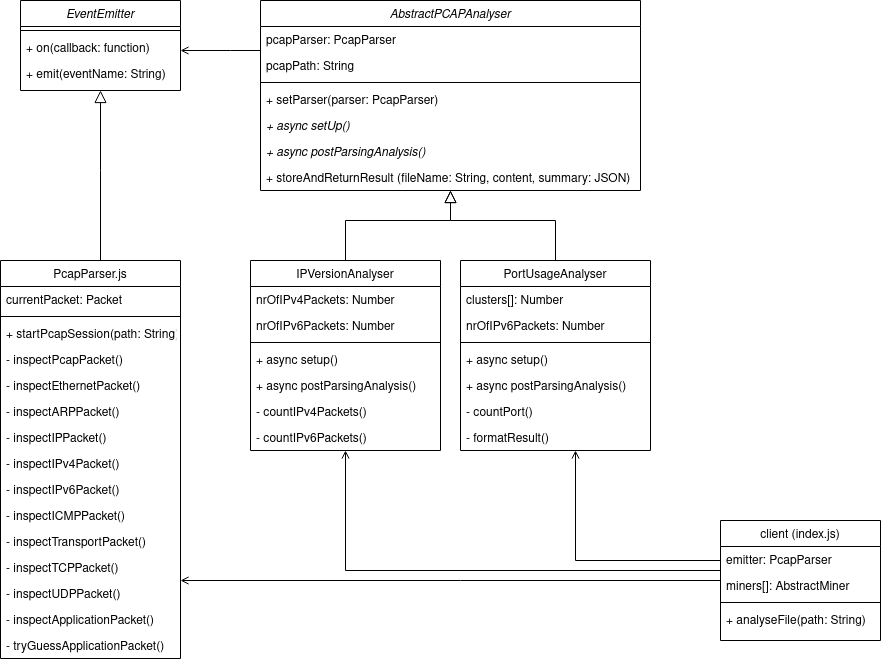
\includegraphics[width=14cm]{images/backend-miners(2).png}
    \caption{Class diagram showing packet decoder, two feature miners and client.}
    \label{fig:classdiagrambackend}
\end{figure}
\subsection{Communication between feature miners and web API}
The previous subsection \ref{orchestratingpacketvisitors} explained how the miner subproject handles the synchronization of different feature miners throughout the mining life cycle. With this in mind, we designed the actual entry point of the feature miner so that multiple front ends can be used. First, the feature miner should be accessible as a CLI tool where one simply provides a parameter pointing to the input file. This posed no challenge since one can simply parse the arguments and invoke the feature miner.
Secondly, it had to be possible to access the feature miner from the web API. Initially, we thought of integrating the feature miner as a module into the web API. Since Node.js only uses a single thread, this can be a problem even when calling the feature miner in an asynchronous manner \cite{nodejs_about}. If the feature miner does CPU-intensive computations, the main thread will be overloaded and the web API will be unable to answer new requests until the feature miner has completed.
The solution to this problem was to make the feature miner aware of how it can communicate with its client. If the feature miner detects that an IPC channel was created from the calling process, it will direct its output to that channel or will otherwise use the \textit{stdout} channel. The former can then be done by forking a child process within the Node.js process of the web api and creating said IPC channel \cite{nodejs_childprocesses}.


 \section{Frontend Development View}
 This section presents the components chosen and thought processes behind choosing them for the front end application the users will interact with. Additionally, it describes how the components are set up hierarchically.
 \subsection{Base Web Application}
 After considering multiple frameworks, it was decided that Vue.js is used as a base framework for the application. Factors that supported this decision was the fact that the authors were familiar with the framework already, meaning they could quickly build a working prototype and the Node.js ecosystem provided many Vue.js-specific modules that made working with it easier. Other frameworks or development methods that were considered included React and templating WebComponents using lit-element. We decided against these two methods, because we did not have any experience using them, meaning a considerable amount of time would have been spent getting familiar with them. While the lit-element/WebComponent approach would have been interesting from a technology standpoint, the ecosystem at the point of writing this report was just not at a point where using it was a hassle-free experience, for example Material Components were not yet fully implemented in WebComponent format.
 
 Vue.js allows the creation of Single Page Applications, which makes the dynamic loading of the applications possible, instead of needing to perform a full web page reload for every action performed. This is supported by a framework-supplied router that matches urls to components and loads them as needed.
 
 For the application to work as a PWA, the necessary manifest and service worker files were created for offline capabilities, as well as icons were created to give a native-like feel to the application, should it be installed on a device.
 
 \subsection{Grid-Layout Engine}
 Since the \emph{Dashboard} component of the application relies on a configurable grid that can re-arrange its tiles automatically, a grid-layouting engine is required. Our requirements for such an engine included:
 \begin{enumerate}
    \item The tiles inside of a grid should be rearrangeable using drag and drop controls.
    \item The vertical size of the grid should be configurable during run-time.
    \item The size of the library should be as small as possible to prevent bloating the front end application's total size.
    \item Sorting and filtering should be supported or built into the library.
    \item The grid should react to changes in the number of tiles, such as deletion of elements and react accordingly, as well as the addition of new tiles.
\end{enumerate}{}
After trying out multiple libraries, such as muuri.js, Gridstack.js and jQuery Shapeshift, a decision was made to use \emph{vue-grid-layout}, since it was the only library that supported dynamically rendering HTML elements that were templated from the persistence layer. This means that other libraries relied on programmatic adding and removing HTML-nodes from the grid, which proved to be difficult since we used templated components that were automatically added and removed to the HTML based on internal state. Another reason why we decided against other libraries was the fact that many relied on jQuery which would have significantly increased application size.
The size and position of the elements is also persisted, meaning programmatic change in location and size of the tiles is also possible.
 \subsection{Components}
 To provide a unified design for the application and prevent us from developing and designing a user interface from scratch, it was decided that reusable components will be used. Since the material design guidelines provide an in-depth explanation on how each available component should be used to build an application that is both familiar to use and visually consistent, it was decided to use a component-library that is styled using material design. Because the framework we used is Vue.js, a requirement was that the components should be supported by or built for Vue.js, so that they can be easily included into the application. We decided to use Vue Material since it enabled us to include only the required components. This was not the case with Vuetify, which is also larger in size overall. The usage of such a library makes it easy to just import for example a tabbed layout without needing to spend unnecessary time configuring CSS and HTML.
 \subsection{Visualization and Charting Libraries}
 At the start of developing the prototype, the goal was to have a simple visualization as a proof-of-concept. This led us to use Chart.js for most of the visualizations, a rather convenient and simple charting library. An alternative would have been D3.js, but we decided against it, since its scope of functionality was much broader than what was intended for our application. This would have resulted in much more configuration for the rather simple visualizations that we intended to implement. This does not mean that a user is restrained to only use Chart.js visualizations from now on. On the contrary, due to our modular approach with feature miners, any method of output can be used, ranging from simple text-based metric displays, to much more complicated 3D-visualizations.
 \subsection{Persistence}
 To persist the data that is worked on in the application, Vue.js' VueX state management library was used. It allows to easily commit and retrieve data from a central storage component throughout the entire application. It also persists data across sessions, by storing the data inside the browser cache, as opposed to just storing it in memory. The persisted data consists of an array of currently opened tiles on the dashboard, whose elements may either be a dataset or a visualization object, which are generically interpreted by the dashboard as tiles. It was necessary to make this array generic, as opposed to two arrays with distinct element types, because the order of elements is important for storing and retrieving setups. Setups are also stored inside VueX, similarily to the currently opened tiles, but annotated with a name and an ID to retrieve them at a later date. 
 \subsection{Component Hierarchy}
 As mentioned previously, the application is made up of three main tabs, \emph{Home}, \emph{Dashboard} and \emph{Datasets}. Illustrated in Figure \ref{fig:frontentHierarchy}, one can see the actual components used for each tab and what data flows between them, i.e. visualization and dataset data.
Starting with the Landing Page, it is not dependant on any component as it just displays static content, i.e. information about the project. The Dashboard tab can contain either data set tiles or visualization tiles, depending on the current setup. On the \emph{Datasets} page, Data Set List Items, as well as the File Upload Form are rendered. The \emph{Dashboard} and \emph{Datasets} pages retrieve and store data to the persistence layer (Named \emph{Store} in the figure), this way data propagation between components is streamlined, as opposed to manually using event emitters and listeners.

\begin{figure}
    \centering
    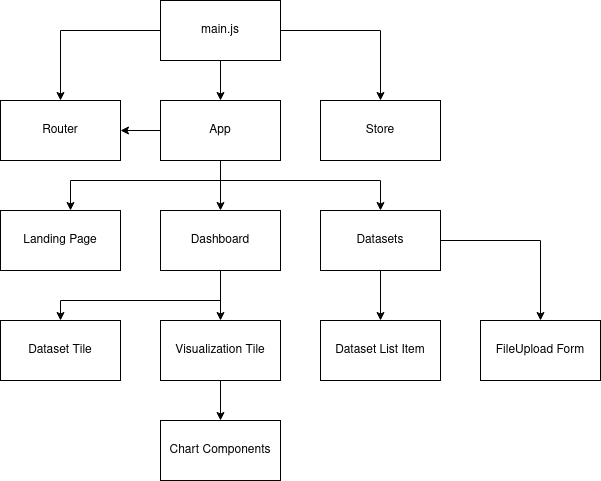
\includegraphics[width=10cm]{images/frontend_hierarchy.png}
    \caption{Component structure of the frontend part of the application.}
    \label{fig:frontentHierarchy}
\end{figure}